\documentclass[a4paper,12pt]{mwart} %{article}
\usepackage[utf8]{inputenc}
\usepackage{polski}
\usepackage{graphicx}


\title{Pracownia 3: ,,Optymalizacja Kodu''}
\author{Mateusz Obara, 264092}

\begin{document}

\maketitle
\thispagestyle{empty}

\subsection*{Informacje o systemie}

\begin{description}
	\item[Dystrybucja:] Fedora 29 64bit
	\item[Jądro systemu:] 5.0.7-200
	\item[Kompilator:] gcc version 8.3.1
	\item[Procesor:] Intel(R) Core(TM) i5 CPU       M 520  @ 2.40GHz
	\item[Liczba rdzeni:] 2, z hyperthreadingiem
\end{description}

\subsection*{Pamięć podręczna}

\begin{description}
	\item[L1d:] 32 KiB, 8-drożny (per rdzeń), rozmiar linii 64 B
	\item[L2:]  256 KiB, 8-drożny (per rdzeń), rozmiar linii 64 B
	\item[L3:] 3 MiB, 12-drożny (współdzielony), rozmiar linii 64 B
\end{description}

\subsection*{Pamięć TLB}

\begin{description}
	\item[L1d:] 4 KiB strony, 4-drożny, 64 wpisy
	\item[L2:] 4 KiB strony, 4-drożny, 512 wpisów
\end{description}

Informacje o pamięciach podręcznych uzyskano na podstawie wydruku programów getconf, x86info oraz cpuid.
\subsection*{Generowanie wyników}
Skrypty rmaker1-1.sh, rmaker1-2.sh, rmaker3-1.sh, rmaker3-2.sh, rmaker4.sh służą do powtórzenia eksperymentu dotyczącego odpowiadającego im zadania i pytania (np rmaker3-2.sh generuje wyniki koniecznie do powiedzi na 2 pytanie w zadaniu 3). Można je również wywołać wszystkie po kolei, za pomocą rmakerall.sh.

Generowanie wyników może trochę zająć, dlatego dołączam również ostatnie wyniki utworzone na mojej maszynie.
\section*{Zadanie 1}

\begin{figure}[h!]
  \includegraphics[width=\linewidth]{graphs/graph1.png}
\end{figure}

\subsection*{Czy wyniki różnią się od tych uzyskanych na slajdzie?}

Tak, różnią się, ale wykazują wspólny trend. Wyniki uzyskane na mojej maszynie wydają się bardziej 'wachać'.

\subsection*{Z czego wynika rozbieżność między wynikami dla poszczególnych wersji mnożenia macierzy?}

Wynika ona z różnej kolejności pobierania danych z pamięci. Szybsze funkcje starają się czytać je tak, aby ograniczyć liczbę missów w cacheu.


\subsection*{Jaki wpływ ma rozmiar kafelka na wydajność multiply?}

\begin{figure}[h!]
  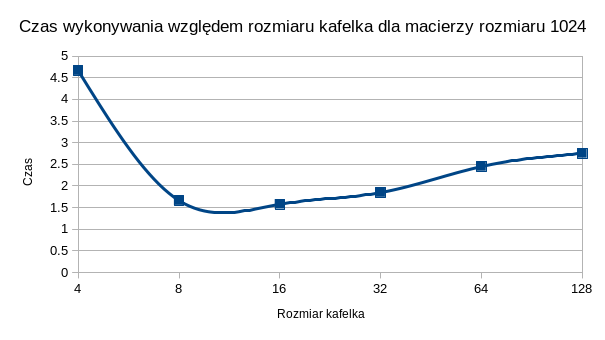
\includegraphics[width=\linewidth]{graphs/graph1-2.png}
\end{figure}

Z danych możemy wyczytać że funkcja działa najszybciej gdy rozmiar kafelka wynosi 16. Kafelek rozmiaru 8 również prezentuje dobre wyniki. Dla reszty, zarówno dla mniejszych i większych wartości obserwujemy dłuższe czasy.



\section*{Zadanie 3}

\subsection*{Jaki wpływ na wydajność transpose2 ma rozmiar kafelka?}

\begin{figure}[h!]
  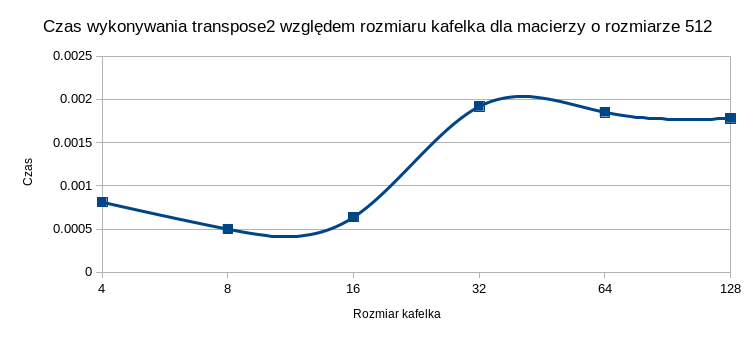
\includegraphics[width=\linewidth]{graphs/graph3-1.png}
\end{figure}

Z zebranych danych wynika że transpose2 jest najwydajniejsza przy kafelku o rozmiarze 8.

\subsection*{Czy czas wykonania programu z różnymi rozmiarami macierzy identyfikuje rozmiary poszczególnych poziomów pamięci podręcznej?}

\begin{figure}[h!]
  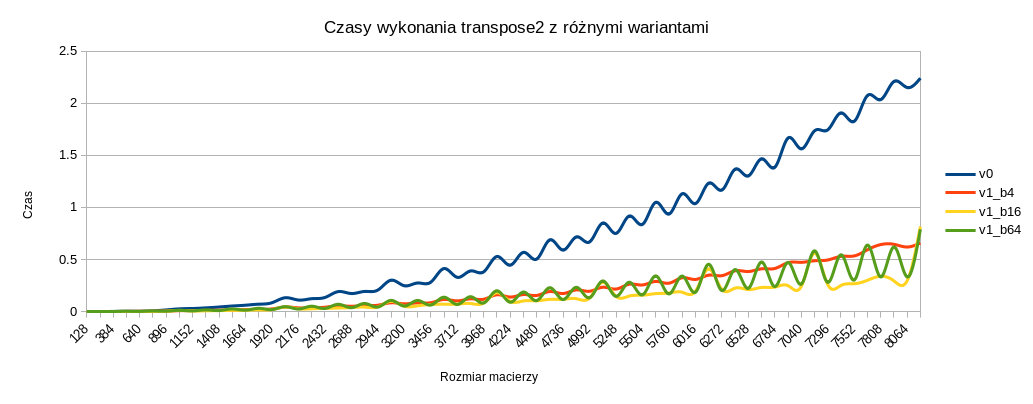
\includegraphics[width=\linewidth]{graphs/graph3-2.png}
\end{figure}

Z wykresu możemy wyczytać cykliczne wzrosty w czasie wykonywania programu. Zauważmy też że wersja bezkafelkowa takich nie posiada. Można zatem wywnioskować że zależne są od kafelków - czyli mniejszych wersji macierzy. O ile można by oszacować rozmiary dla L1 i L2, L3 jest współdzielona i pozostaje problemem.

\section*{Zadanie 4}


\subsection*{Ile instrukcji maszynowych ma ciało pętli przed i po optymalizacji?}

Przed optymalizacją: 57
Po optymalizacji: 58

\subsection*{Ile spośród nich to instrukcje warunkowe?}

Przed optymalizacją: 6
Po optymalizacji: 3

\subsection*{Czy rozmiar tablicy ma duży wpływ na działanie programu?}

\begin{figure}[h!]
  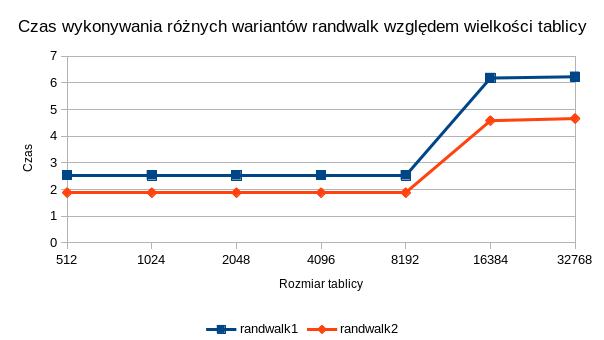
\includegraphics[width=\linewidth]{graphs/graph4.png}
\end{figure}


Tak. podążając za wykresem, widzimy że na początku, dla dużej ilości danych czas wykonywania funkcji nie zmienia się znacznie. Jednak, na rozmiarze 16384 zauważamy znaczny skok, a następnie znów niewieką zmianę. Wspomniany wzrost sugeruje że czas wykonywania randwalk jest jednak zależny od rozmiaru tablicy.

\end{document}
